\documentclass[twoside]{book}

% Packages required by doxygen
\usepackage{fixltx2e}
\usepackage{calc}
\usepackage{doxygen}
\usepackage[export]{adjustbox} % also loads graphicx
\usepackage{graphicx}
\usepackage[utf8]{inputenc}
\usepackage{makeidx}
\usepackage{multicol}
\usepackage{multirow}
\PassOptionsToPackage{warn}{textcomp}
\usepackage{textcomp}
\usepackage[nointegrals]{wasysym}
\usepackage[table]{xcolor}

% NLS support packages
\usepackage[brazil]{babel}
% Font selection
\usepackage[T1]{fontenc}
\usepackage[scaled=.90]{helvet}
\usepackage{courier}
\usepackage{amssymb}
\usepackage{sectsty}
\renewcommand{\familydefault}{\sfdefault}
\allsectionsfont{%
  \fontseries{bc}\selectfont%
  \color{darkgray}%
}
\renewcommand{\DoxyLabelFont}{%
  \fontseries{bc}\selectfont%
  \color{darkgray}%
}
\newcommand{\+}{\discretionary{\mbox{\scriptsize$\hookleftarrow$}}{}{}}

% Page & text layout
\usepackage{geometry}
\geometry{%
  a4paper,%
  top=2.5cm,%
  bottom=2.5cm,%
  left=2.5cm,%
  right=2.5cm%
}
\tolerance=750
\hfuzz=15pt
\hbadness=750
\setlength{\emergencystretch}{15pt}
\setlength{\parindent}{0cm}
\setlength{\parskip}{3ex plus 2ex minus 2ex}
\makeatletter
\renewcommand{\paragraph}{%
  \@startsection{paragraph}{4}{0ex}{-1.0ex}{1.0ex}{%
    \normalfont\normalsize\bfseries\SS@parafont%
  }%
}
\renewcommand{\subparagraph}{%
  \@startsection{subparagraph}{5}{0ex}{-1.0ex}{1.0ex}{%
    \normalfont\normalsize\bfseries\SS@subparafont%
  }%
}
\makeatother

% Headers & footers
\usepackage{fancyhdr}
\pagestyle{fancyplain}
\fancyhead[LE]{\fancyplain{}{\bfseries\thepage}}
\fancyhead[CE]{\fancyplain{}{}}
\fancyhead[RE]{\fancyplain{}{\bfseries\leftmark}}
\fancyhead[LO]{\fancyplain{}{\bfseries\rightmark}}
\fancyhead[CO]{\fancyplain{}{}}
\fancyhead[RO]{\fancyplain{}{\bfseries\thepage}}
\fancyfoot[LE]{\fancyplain{}{}}
\fancyfoot[CE]{\fancyplain{}{}}
\fancyfoot[RE]{\fancyplain{}{\bfseries\scriptsize Gerado por Doxygen }}
\fancyfoot[LO]{\fancyplain{}{\bfseries\scriptsize Gerado por Doxygen }}
\fancyfoot[CO]{\fancyplain{}{}}
\fancyfoot[RO]{\fancyplain{}{}}
\renewcommand{\footrulewidth}{0.4pt}
\renewcommand{\chaptermark}[1]{%
  \markboth{#1}{}%
}
\renewcommand{\sectionmark}[1]{%
  \markright{\thesection\ #1}%
}

% Indices & bibliography
\usepackage{natbib}
\usepackage[titles]{tocloft}
\setcounter{tocdepth}{3}
\setcounter{secnumdepth}{5}
\makeindex

% Hyperlinks (required, but should be loaded last)
\usepackage{ifpdf}
\ifpdf
  \usepackage[pdftex,pagebackref=true]{hyperref}
\else
  \usepackage[ps2pdf,pagebackref=true]{hyperref}
\fi
\hypersetup{%
  colorlinks=true,%
  linkcolor=blue,%
  citecolor=blue,%
  unicode%
}

% Custom commands
\newcommand{\clearemptydoublepage}{%
  \newpage{\pagestyle{empty}\cleardoublepage}%
}

\usepackage{caption}
\captionsetup{labelsep=space,justification=centering,font={bf},singlelinecheck=off,skip=4pt,position=top}

%===== C O N T E N T S =====

\begin{document}

% Titlepage & ToC
\hypersetup{pageanchor=false,
             bookmarksnumbered=true,
             pdfencoding=unicode
            }
\pagenumbering{alph}
\begin{titlepage}
\vspace*{7cm}
\begin{center}%
{\Large Produtor \\[1ex]\large 0.\+0.\+0.\+1 }\\
\vspace*{1cm}
{\large Gerado por Doxygen 1.8.13}\\
\end{center}
\end{titlepage}
\clearemptydoublepage
\pagenumbering{roman}
\tableofcontents
\clearemptydoublepage
\pagenumbering{arabic}
\hypersetup{pageanchor=true}

%--- Begin generated contents ---
\chapter{Namespaces}
\section{Lista de Namespaces}
Esta é a lista de todos os Namespaces com suas respectivas descrições\+:\begin{DoxyCompactList}
\item\contentsline{section}{\hyperlink{namespace_ui}{Ui} }{\pageref{namespace_ui}}{}
\end{DoxyCompactList}

\chapter{Índice Hierárquico}
\section{Hierarquia de Classes}
Esta lista de hierarquias está parcialmente ordenada (ordem alfabética)\+:\begin{DoxyCompactList}
\item Q\+Main\+Window\begin{DoxyCompactList}
\item \contentsline{section}{Main\+Window}{\pageref{class_main_window}}{}
\end{DoxyCompactList}
\end{DoxyCompactList}

\chapter{Índice dos Componentes}
\section{Lista de Componentes}
Aqui estão as classes, estruturas, uniões e interfaces e suas respectivas descrições\+:\begin{DoxyCompactList}
\item\contentsline{section}{\hyperlink{class_main_window}{Main\+Window} }{\pageref{class_main_window}}{}
\end{DoxyCompactList}

\chapter{Índice dos Arquivos}
\section{Lista de Arquivos}
Esta é a lista de todos os arquivos e suas respectivas descrições\+:\begin{DoxyCompactList}
\item\contentsline{section}{\hyperlink{main_8cpp}{main.\+cpp} }{\pageref{main_8cpp}}{}
\item\contentsline{section}{\hyperlink{mainwindow_8cpp}{mainwindow.\+cpp} }{\pageref{mainwindow_8cpp}}{}
\item\contentsline{section}{\hyperlink{mainwindow_8h}{mainwindow.\+h} }{\pageref{mainwindow_8h}}{}
\end{DoxyCompactList}

\chapter{Namespaces}
\hypertarget{namespace_ui}{}\section{Refência do Namespace Ui}
\label{namespace_ui}\index{Ui@{Ui}}

\chapter{Classes}
\hypertarget{class_main_window}{}\section{Referência da Classe Main\+Window}
\label{class_main_window}\index{Main\+Window@{Main\+Window}}


{\ttfamily \#include $<$mainwindow.\+h$>$}

Diagrama de Hierarquia para Main\+Window\+:\begin{figure}[H]
\begin{center}
\leavevmode
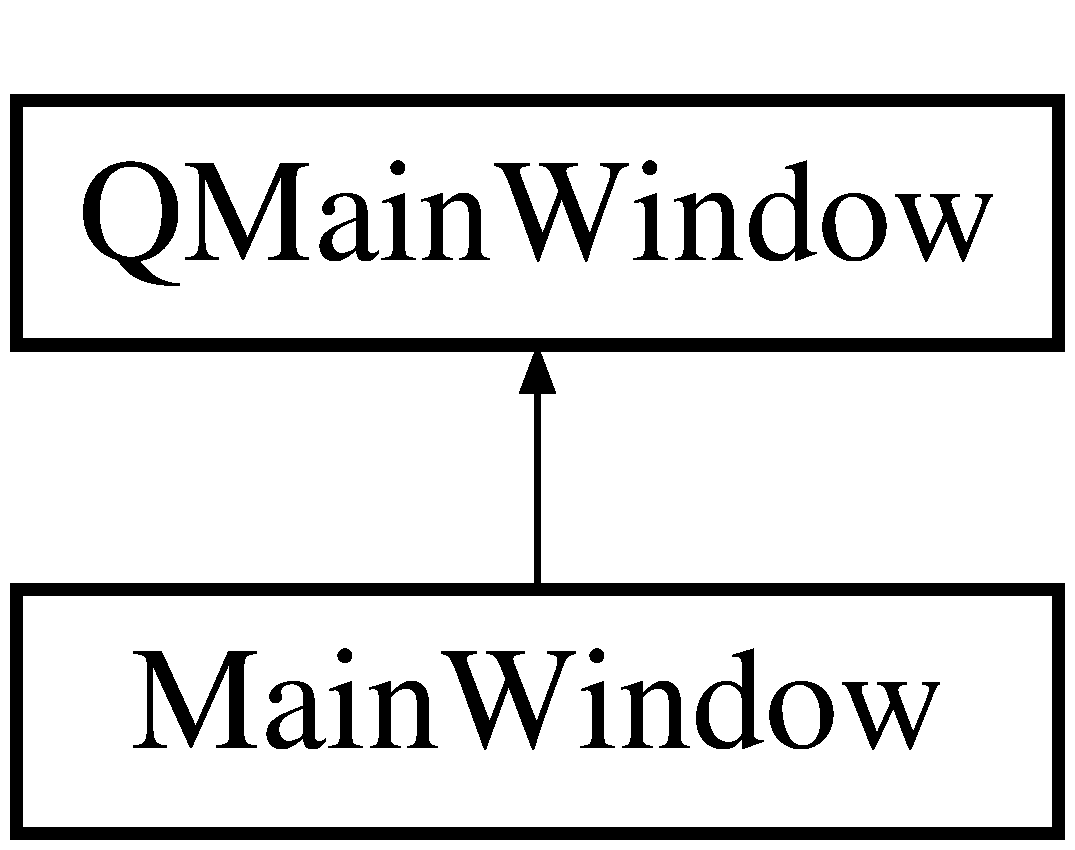
\includegraphics[height=2.000000cm]{class_main_window}
\end{center}
\end{figure}
\subsection*{Slots Públicos}
\begin{DoxyCompactItemize}
\item 
void \hyperlink{class_main_window_afdfeb13ec363b0eb8ecacaf0aa13b605}{put\+Data} ()
\begin{DoxyCompactList}\small\item\em Slot produtor de dados. \end{DoxyCompactList}\item 
void \hyperlink{class_main_window_afd17285381f6457c552f26f359f8f968}{connecting} ()
\begin{DoxyCompactList}\small\item\em Slot de chamada da conexao. \end{DoxyCompactList}\item 
void \hyperlink{class_main_window_a496a126baa8c2a0a7d0bdab86c128f98}{disconnecting} ()
\begin{DoxyCompactList}\small\item\em Slot de desconexao. \end{DoxyCompactList}\item 
void \hyperlink{class_main_window_a9d08a694a5f9c532225754381b8011ea}{timer\+Event} (Q\+Timer\+Event $\ast$e)
\begin{DoxyCompactList}\small\item\em Chamada do evento temporario. \end{DoxyCompactList}\item 
void \hyperlink{class_main_window_a756fd5832a55713567189c43d8aa27ca}{starting} ()
\begin{DoxyCompactList}\small\item\em Slot que inicia o timer. \end{DoxyCompactList}\item 
void \hyperlink{class_main_window_a6ba0902dc1552226ae4a7866a42efee0}{stopping} ()
\begin{DoxyCompactList}\small\item\em Slot que mata o timer. \end{DoxyCompactList}\end{DoxyCompactItemize}
\subsection*{Métodos Públicos}
\begin{DoxyCompactItemize}
\item 
\hyperlink{class_main_window_a8b244be8b7b7db1b08de2a2acb9409db}{Main\+Window} (Q\+Widget $\ast$parent=0)
\begin{DoxyCompactList}\small\item\em Construtor da classe. \end{DoxyCompactList}\item 
\hyperlink{class_main_window_ae98d00a93bc118200eeef9f9bba1dba7}{$\sim$\+Main\+Window} ()
\begin{DoxyCompactList}\small\item\em Destrutor da classe. \end{DoxyCompactList}\item 
void \hyperlink{class_main_window_ac5b669957c442b6eb68573dacfce33e1}{tcp\+Connect} ()
\begin{DoxyCompactList}\small\item\em Slot de conexao. \end{DoxyCompactList}\end{DoxyCompactItemize}
\subsection*{Atributos Públicos}
\begin{DoxyCompactItemize}
\item 
Q\+Timer $\ast$ \hyperlink{class_main_window_a356578805ed1248a7f2807434cb0e5ee}{timer}
\end{DoxyCompactItemize}


\subsection{Construtores \& Destrutores}
\mbox{\Hypertarget{class_main_window_a8b244be8b7b7db1b08de2a2acb9409db}\label{class_main_window_a8b244be8b7b7db1b08de2a2acb9409db}} 
\index{Main\+Window@{Main\+Window}!Main\+Window@{Main\+Window}}
\index{Main\+Window@{Main\+Window}!Main\+Window@{Main\+Window}}
\subsubsection{\texorpdfstring{Main\+Window()}{MainWindow()}}
{\footnotesize\ttfamily Main\+Window\+::\+Main\+Window (\begin{DoxyParamCaption}\item[{Q\+Widget $\ast$}]{parent = {\ttfamily 0} }\end{DoxyParamCaption})\hspace{0.3cm}{\ttfamily [explicit]}}



Construtor da classe. 

Construtor da classe \hyperlink{class_main_window}{Main\+Window} que inicializa o objeto
\begin{DoxyCode}
8                                       :
9   QMainWindow(parent), ui(\textcolor{keyword}{new} Ui::MainWindow)\{
13   ui->setupUi(\textcolor{keyword}{this});
14   socket = \textcolor{keyword}{new} QTcpSocket(\textcolor{keyword}{this});
15   \textcolor{keywordtype}{id} = 0;
16 \}
\end{DoxyCode}
\mbox{\Hypertarget{class_main_window_ae98d00a93bc118200eeef9f9bba1dba7}\label{class_main_window_ae98d00a93bc118200eeef9f9bba1dba7}} 
\index{Main\+Window@{Main\+Window}!````~Main\+Window@{$\sim$\+Main\+Window}}
\index{````~Main\+Window@{$\sim$\+Main\+Window}!Main\+Window@{Main\+Window}}
\subsubsection{\texorpdfstring{$\sim$\+Main\+Window()}{~MainWindow()}}
{\footnotesize\ttfamily Main\+Window\+::$\sim$\+Main\+Window (\begin{DoxyParamCaption}{ }\end{DoxyParamCaption})}



Destrutor da classe. 

Deleta os objetos alocados dinamicamnete
\begin{DoxyCode}
132                        \{
136   \textcolor{keyword}{delete} socket;
137   \textcolor{keyword}{delete} ui;
138 \}
\end{DoxyCode}


\subsection{Métodos}
\mbox{\Hypertarget{class_main_window_afd17285381f6457c552f26f359f8f968}\label{class_main_window_afd17285381f6457c552f26f359f8f968}} 
\index{Main\+Window@{Main\+Window}!connecting@{connecting}}
\index{connecting@{connecting}!Main\+Window@{Main\+Window}}
\subsubsection{\texorpdfstring{connecting}{connecting}}
{\footnotesize\ttfamily void Main\+Window\+::connecting (\begin{DoxyParamCaption}{ }\end{DoxyParamCaption})\hspace{0.3cm}{\ttfamily [slot]}}



Slot de chamada da conexao. 

Slot que chama a conexao
\begin{DoxyCode}
82                            \{
86     \hyperlink{class_main_window_ac5b669957c442b6eb68573dacfce33e1}{tcpConnect}();
87 \}
\end{DoxyCode}
\mbox{\Hypertarget{class_main_window_a496a126baa8c2a0a7d0bdab86c128f98}\label{class_main_window_a496a126baa8c2a0a7d0bdab86c128f98}} 
\index{Main\+Window@{Main\+Window}!disconnecting@{disconnecting}}
\index{disconnecting@{disconnecting}!Main\+Window@{Main\+Window}}
\subsubsection{\texorpdfstring{disconnecting}{disconnecting}}
{\footnotesize\ttfamily void Main\+Window\+::disconnecting (\begin{DoxyParamCaption}{ }\end{DoxyParamCaption})\hspace{0.3cm}{\ttfamily [slot]}}



Slot de desconexao. 

Slot que desconecta o produtor do servidor
\begin{DoxyCode}
90                               \{
94     socket->disconnectFromHost();
95     qDebug() << \textcolor{stringliteral}{"Disconnected"};
96 \}
\end{DoxyCode}
\mbox{\Hypertarget{class_main_window_afdfeb13ec363b0eb8ecacaf0aa13b605}\label{class_main_window_afdfeb13ec363b0eb8ecacaf0aa13b605}} 
\index{Main\+Window@{Main\+Window}!put\+Data@{put\+Data}}
\index{put\+Data@{put\+Data}!Main\+Window@{Main\+Window}}
\subsubsection{\texorpdfstring{put\+Data}{putData}}
{\footnotesize\ttfamily void Main\+Window\+::put\+Data (\begin{DoxyParamCaption}{ }\end{DoxyParamCaption})\hspace{0.3cm}{\ttfamily [slot]}}



Slot produtor de dados. 

Envia dados gerados aleatoriamente para o servidor
\begin{DoxyCode}
34                         \{
38   QString str;
39   qint64 msecdate;
40   QString random;
41   QString datenumber;
42   \textcolor{keywordtype}{int} interval;
43   \textcolor{keywordtype}{int} numRand;
44   \textcolor{keywordtype}{int} min;
45   \textcolor{keywordtype}{int} max;
46 
47   min = ui->horizontalSlider\_Min->sliderPosition();
48   max = ui->horizontalSlider\_Max->sliderPosition();
49 
50   \textcolor{keywordflow}{if}(max>min)\{
51     interval = max - min + 1;
52     numRand = (qrand()%interval) + (min);
53   \}
54   \textcolor{keywordflow}{else} \textcolor{keywordflow}{if}(min>max)\{
55     interval = min - max + 1;
56     numRand = (qrand()%interval) + (max);
57   \}
58   \textcolor{keywordflow}{else}
59       numRand = 0;
60 
61   random = QString::number(numRand);
62 
63 
64   \textcolor{keywordflow}{if}(socket->state()== QAbstractSocket::ConnectedState)\{
65 
66     msecdate = QDateTime::currentDateTime().toMSecsSinceEpoch();
67     datenumber = QString::number(msecdate);
68     str = \textcolor{stringliteral}{"set "}+ datenumber + \textcolor{stringliteral}{" "} + random +\textcolor{stringliteral}{"\(\backslash\)r\(\backslash\)n"};
69 
70 
71 
72       qDebug() << str;
73       qDebug() << socket->write(str.toStdString().c\_str()) << \textcolor{stringliteral}{" bytes written"};
74       \textcolor{keywordflow}{if}(socket->waitForBytesWritten(3000))\{
75         qDebug() << \textcolor{stringliteral}{"wrote - "} << id;
76       \}
77   \}
78   ui->textBrowser->append(str);
79 \}
\end{DoxyCode}
\mbox{\Hypertarget{class_main_window_a756fd5832a55713567189c43d8aa27ca}\label{class_main_window_a756fd5832a55713567189c43d8aa27ca}} 
\index{Main\+Window@{Main\+Window}!starting@{starting}}
\index{starting@{starting}!Main\+Window@{Main\+Window}}
\subsubsection{\texorpdfstring{starting}{starting}}
{\footnotesize\ttfamily void Main\+Window\+::starting (\begin{DoxyParamCaption}{ }\end{DoxyParamCaption})\hspace{0.3cm}{\ttfamily [slot]}}



Slot que inicia o timer. 

Inicia o timer que determinara o periodo de repeticao dos eventos
\begin{DoxyCode}
108                          \{
112     \textcolor{keywordflow}{if}(\textcolor{keywordtype}{id}==0)\{
113         startTimer(ui->horizontalSlider\_Timing->value()*1000);
114     \}
115     \textcolor{keywordflow}{else}\{
116         killTimer(\textcolor{keywordtype}{id});
117         startTimer(ui->horizontalSlider\_Timing->value()*1000);
118     \}
119 \}
\end{DoxyCode}
\mbox{\Hypertarget{class_main_window_a6ba0902dc1552226ae4a7866a42efee0}\label{class_main_window_a6ba0902dc1552226ae4a7866a42efee0}} 
\index{Main\+Window@{Main\+Window}!stopping@{stopping}}
\index{stopping@{stopping}!Main\+Window@{Main\+Window}}
\subsubsection{\texorpdfstring{stopping}{stopping}}
{\footnotesize\ttfamily void Main\+Window\+::stopping (\begin{DoxyParamCaption}{ }\end{DoxyParamCaption})\hspace{0.3cm}{\ttfamily [slot]}}



Slot que mata o timer. 

Finaliza o timer que estiver atuando
\begin{DoxyCode}
123                          \{
127     killTimer(\textcolor{keywordtype}{id});
128     \textcolor{keywordtype}{id} = 0;
129 \}
\end{DoxyCode}
\mbox{\Hypertarget{class_main_window_ac5b669957c442b6eb68573dacfce33e1}\label{class_main_window_ac5b669957c442b6eb68573dacfce33e1}} 
\index{Main\+Window@{Main\+Window}!tcp\+Connect@{tcp\+Connect}}
\index{tcp\+Connect@{tcp\+Connect}!Main\+Window@{Main\+Window}}
\subsubsection{\texorpdfstring{tcp\+Connect()}{tcpConnect()}}
{\footnotesize\ttfamily void Main\+Window\+::tcp\+Connect (\begin{DoxyParamCaption}{ }\end{DoxyParamCaption})}



Slot de conexao. 

Slot que conecta o produtor de dados ao servidor
\begin{DoxyCode}
19                            \{
23     qDebug() << ui->lineEdit\_ip->text();
24   socket->connectToHost(ui->lineEdit\_ip->text(),1234);
25   \textcolor{keywordflow}{if}(socket->waitForConnected(3000))\{
26     qDebug() << \textcolor{stringliteral}{"Connected"};
27   \}
28   \textcolor{keywordflow}{else}\{
29     qDebug() << \textcolor{stringliteral}{"Disconnected"};
30   \}
31 \}
\end{DoxyCode}
\mbox{\Hypertarget{class_main_window_a9d08a694a5f9c532225754381b8011ea}\label{class_main_window_a9d08a694a5f9c532225754381b8011ea}} 
\index{Main\+Window@{Main\+Window}!timer\+Event@{timer\+Event}}
\index{timer\+Event@{timer\+Event}!Main\+Window@{Main\+Window}}
\subsubsection{\texorpdfstring{timer\+Event}{timerEvent}}
{\footnotesize\ttfamily void Main\+Window\+::timer\+Event (\begin{DoxyParamCaption}\item[{Q\+Timer\+Event $\ast$}]{e }\end{DoxyParamCaption})\hspace{0.3cm}{\ttfamily [slot]}}



Chamada do evento temporario. 

Slot que, periodicamente, chama a funcao de producao de dados
\begin{DoxyCode}
99                                          \{
103     \hyperlink{class_main_window_afdfeb13ec363b0eb8ecacaf0aa13b605}{putData}();
104     \textcolor{keywordtype}{id} = e->timerId();
105 \}
\end{DoxyCode}


\subsection{Atributos}
\mbox{\Hypertarget{class_main_window_a356578805ed1248a7f2807434cb0e5ee}\label{class_main_window_a356578805ed1248a7f2807434cb0e5ee}} 
\index{Main\+Window@{Main\+Window}!timer@{timer}}
\index{timer@{timer}!Main\+Window@{Main\+Window}}
\subsubsection{\texorpdfstring{timer}{timer}}
{\footnotesize\ttfamily Q\+Timer$\ast$ Main\+Window\+::timer}



A documentação para esta classe foi gerada a partir dos seguintes arquivos\+:\begin{DoxyCompactItemize}
\item 
\hyperlink{mainwindow_8h}{mainwindow.\+h}\item 
\hyperlink{mainwindow_8cpp}{mainwindow.\+cpp}\end{DoxyCompactItemize}

\chapter{Arquivos}
\hypertarget{main_8cpp}{}\section{Referência do Arquivo main.\+cpp}
\label{main_8cpp}\index{main.\+cpp@{main.\+cpp}}
{\ttfamily \#include \char`\"{}mainwindow.\+h\char`\"{}}\newline
{\ttfamily \#include $<$Q\+Application$>$}\newline
\subsection*{Funções}
\begin{DoxyCompactItemize}
\item 
int \hyperlink{main_8cpp_a0ddf1224851353fc92bfbff6f499fa97}{main} (int argc, char $\ast$argv\mbox{[}$\,$\mbox{]})
\end{DoxyCompactItemize}


\subsection{Funções}
\mbox{\Hypertarget{main_8cpp_a0ddf1224851353fc92bfbff6f499fa97}\label{main_8cpp_a0ddf1224851353fc92bfbff6f499fa97}} 
\index{main.\+cpp@{main.\+cpp}!main@{main}}
\index{main@{main}!main.\+cpp@{main.\+cpp}}
\subsubsection{\texorpdfstring{main()}{main()}}
{\footnotesize\ttfamily int main (\begin{DoxyParamCaption}\item[{int}]{argc,  }\item[{char $\ast$}]{argv\mbox{[}$\,$\mbox{]} }\end{DoxyParamCaption})}


\begin{DoxyCode}
5 \{
6   QApplication a(argc, argv);
7   \hyperlink{class_main_window}{MainWindow} w;
8   w.show();
9 
10   \textcolor{keywordflow}{return} a.exec();
11 \}
\end{DoxyCode}

\hypertarget{mainwindow_8cpp}{}\section{Referência do Arquivo mainwindow.\+cpp}
\label{mainwindow_8cpp}\index{mainwindow.\+cpp@{mainwindow.\+cpp}}
{\ttfamily \#include \char`\"{}mainwindow.\+h\char`\"{}}\newline
{\ttfamily \#include \char`\"{}ui\+\_\+mainwindow.\+h\char`\"{}}\newline
{\ttfamily \#include $<$Q\+Date\+Time$>$}\newline
{\ttfamily \#include $<$Q\+String$>$}\newline
{\ttfamily \#include $<$Q\+Timer$>$}\newline

\hypertarget{mainwindow_8h}{}\section{Referência do Arquivo mainwindow.\+h}
\label{mainwindow_8h}\index{mainwindow.\+h@{mainwindow.\+h}}
{\ttfamily \#include $<$Q\+Main\+Window$>$}\newline
{\ttfamily \#include $<$Q\+Tcp\+Socket$>$}\newline
{\ttfamily \#include $<$Q\+Debug$>$}\newline
{\ttfamily \#include $<$Q\+Timer$>$}\newline
\subsection*{Componentes}
\begin{DoxyCompactItemize}
\item 
class \hyperlink{class_main_window}{Main\+Window}
\end{DoxyCompactItemize}
\subsection*{Namespaces}
\begin{DoxyCompactItemize}
\item 
 \hyperlink{namespace_ui}{Ui}
\end{DoxyCompactItemize}

%--- End generated contents ---

% Index
\backmatter
\newpage
\phantomsection
\clearemptydoublepage
\addcontentsline{toc}{chapter}{Índice}
\printindex

\end{document}
